\section{Critical Levels}

There are around 500 different layers, and XXX regions in a single segmentation tree. Besides, regions in nearby layer can be highly similar. Assessing all of them is both unnecessary and computationally impractical. Therefore, as a pre-processing step, we aim to predict a set of critical levels. These critical levels should be complementary to achieve a high recall to ground truth regions, yet keep the size of set smaller. Similar idea was used in~\cite{krahenbuhl2014geodesic}, where they use critical levels to predict size of segmentation masks.

In order to identify these critical levels efficiently, we train a model based on segmentation entropy features. Segmentation entropy of a segmentation $S$ is defined as:
\begin{equation}
Entropy(S) = \sum_{\textbf{r}\in S}{|\textbf{r}|log(|\textbf{r}|)}
\end{equation}

$|\textbf{r}|$ represents the area of a region $\textbf{r}$ in segmentation $S$. Since only the area is required, segmentation entropy is very fast to compute. It enables us to assess difference between layers of a segmentation tree efficiently, as illustrated in Fig~\ref{fig:entropy}. The steep point on the curve indicates there is a large change in the segmentation.

\begin{figure}
\begin{center}
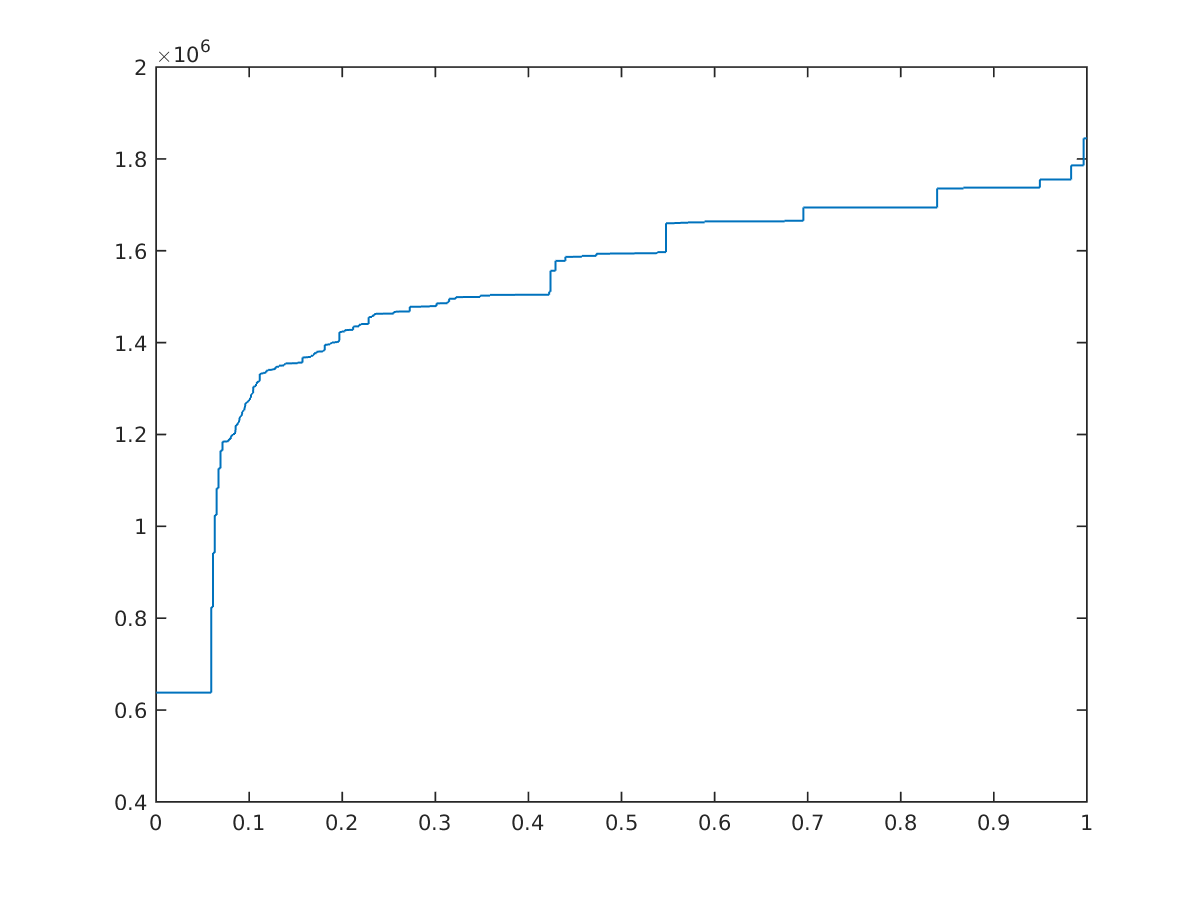
\includegraphics[width=0.5\linewidth]{fig/6046_ucm.png}
\end{center}
\caption{entropy}
\label{fig:entropy}
\end{figure}

The features used includes: value of threshold and entropy, and local gradient of both threshold and entropy calculated with different footstep length. More details about the feature are in the supplementary materials.

\yh{Experiments are not done, will add later}
  